
% Set the color of hyperlinks (e.g., TOC links, URLs) to white so they are not visible
\hypersetup{
  colorlinks=white,
  linkcolor=white,     % Color of internal links (e.g., section references)
  urlcolor=white       % Color of URLs
}

% Create a full-screen frame without any standard header/footer
\begin{frame}[plain]
  % Overlay allows drawing over the whole slide
  \begin{tikzpicture}[overlay, remember picture]

  % Define two points A and B to span the area for the background rectangle
  \node[] (A) at (-2.5,2){};    % Top-left corner of the background
  \node[] (B) at (15, -4){};    % Bottom-right corner of the background

  % Draw a large blue rectangle for the background
  \fill[color=renatoSblue!90] (A) rectangle (B);

  % Insert the hexacopter image at a fixed position relative to point A
  \node[anchor=north west, xshift= 0cm, yshift=0.4cm] at ($(A)+(8,0)$) {
    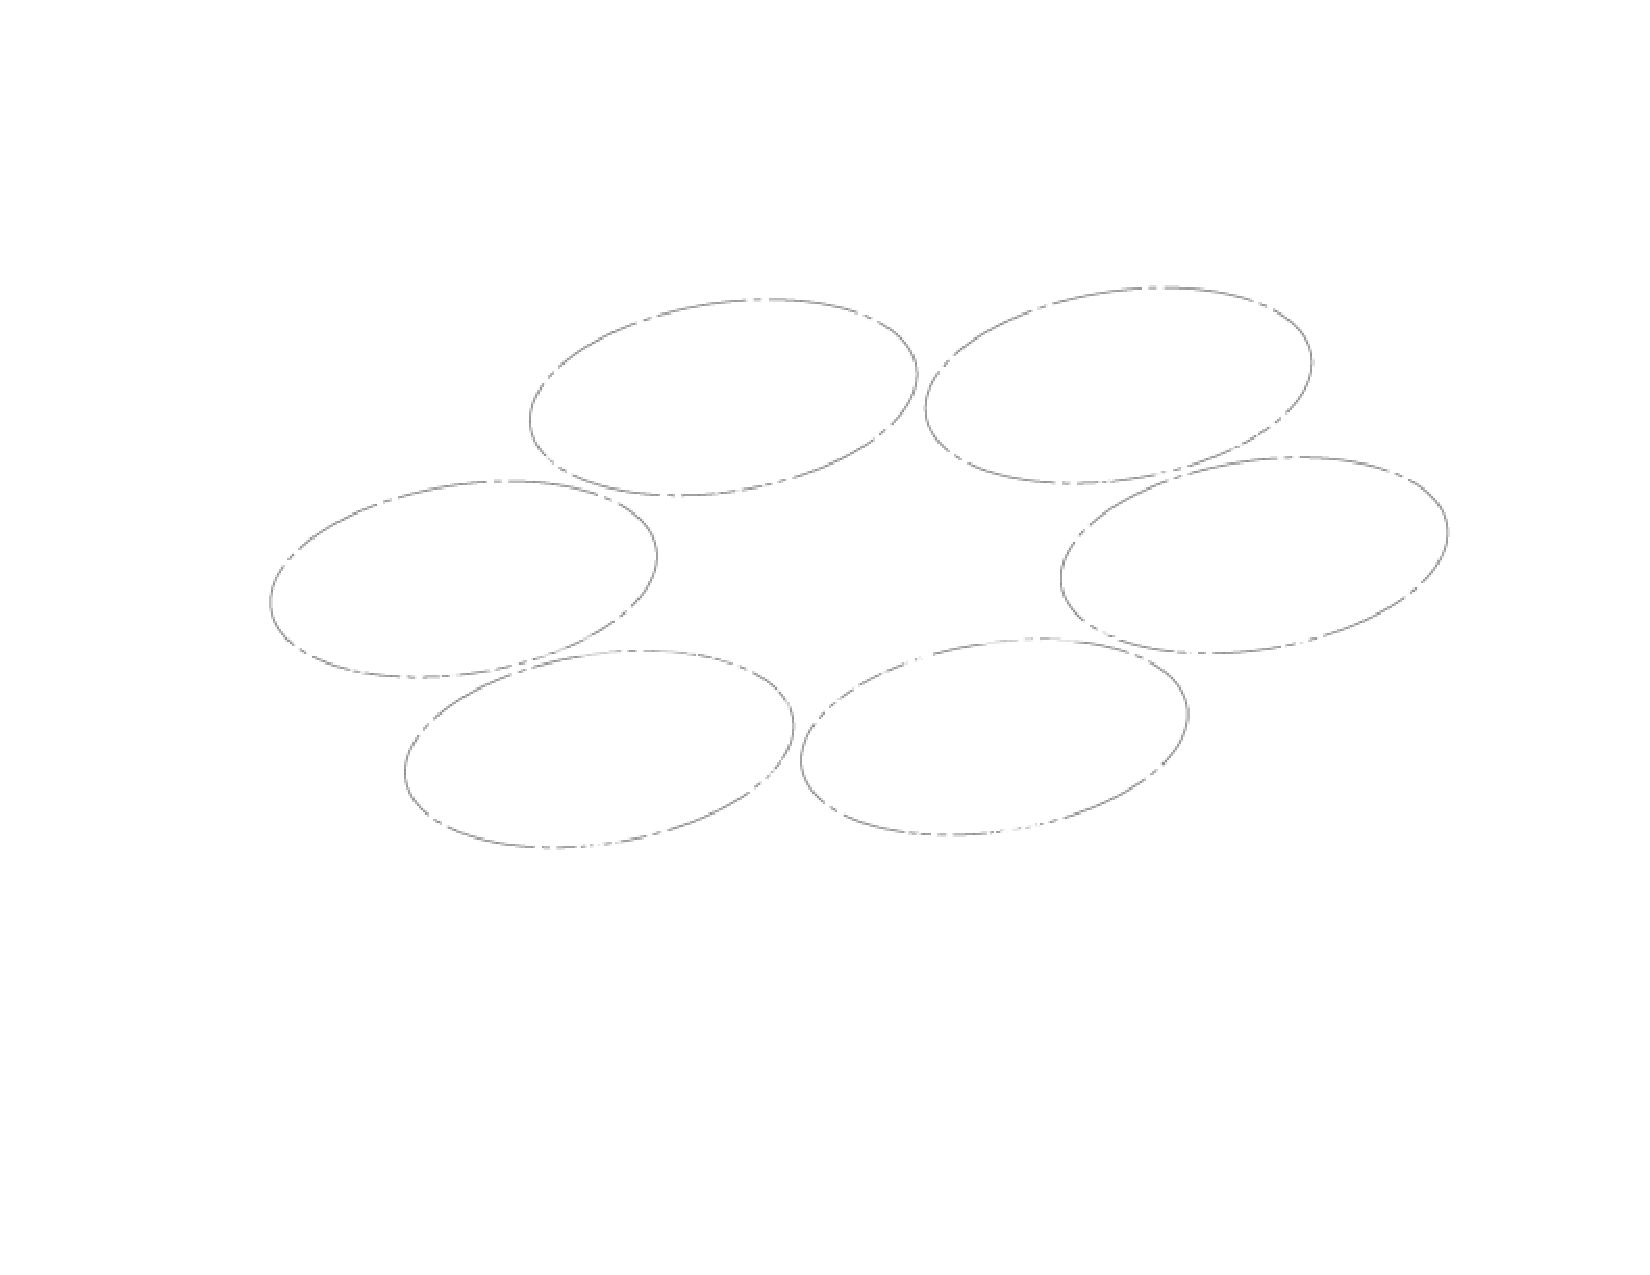
\includegraphics[width=0.7\textwidth]{figures/hexacopter_white.pdf}
  };

  % Insert the University of Stuttgart logo at the top-left of the slide
  \node[anchor=north west] (UNI) at ([xshift=0.5cm, yshift=-2cm]current page.north west) {\pgfuseimage{unilogow}};
  
  % Add the name of the institute next to the logo
  \node[text=white, font=\normalsize, anchor=west] at ($(UNI.west) + (1.25,-0.35)$) {Institut für Flugmechanik und Flugregelung};  
    
  % Insert the title at the bottom-left of the slide
  \node[text=white, anchor=west] at ([yshift=4cm, xshift=0.5cm]current page.south west) {
    \begin{minipage}{0.5\textwidth}
      \raggedright \title   % Title variable
    \end{minipage}  
  };
  
  % Add a subtitle line
  \node[text=white, font=\small, anchor=west] at ([yshift=3.2cm, xshift=0.5cm]current page.south west) {System Theoretical Methods for Flight Control};  

  % Add the actual subtitle defined by \subtitle
  \node[text=white, font=\huge, anchor=west] at ([yshift=2.8cm, xshift=0.5cm]current page.south west) {\subtitle};  
  
  % Add the short author name defined by \shortauthor
  \node[text=white, font=\large, anchor=west] at ([yshift=2.2cm, xshift=0.5cm]current page.south west) {\shortauthor};

  \end{tikzpicture}
\end{frame}

% Set Beamer color for frame titles in the rest of the document
\setbeamercolor{frametitle}{fg=Blue,bg=LightGrey}